\documentclass[aspectratio=169,10pt]{beamer}
\usepackage[T1]{fontenc}
\usepackage[utf8]{inputenc}
\usepackage[spanish,es-nodecimaldot]{babel}
\usepackage{lmodern}
\usepackage{amsmath}
\usepackage{booktabs}
\usepackage{graphicx}
\usepackage{tikz}
\usetikzlibrary{arrows.meta,positioning,babel}

% ============================================================
% DATOS DE LA PORTADA (revisar antes de compilar)
% ============================================================
\newcommand{\subtitulo}{Tesis de licenciatura}
\newcommand{\correo}{a335951@uach.mx}
\newcommand{\fecha}{27 de noviembre de 2026}
% Si aplica, descomentar y completar la línea del profesor o director:
\newcommand{\lineaprofesor}{}
% \newcommand{\lineaprofesor}{{\small Director: NOMBRE\quad \texttt{correo@uach.mx}}}

% ============================================================
% TEMA
% ============================================================
\usetheme{Madrid}
\definecolor{azulfi}{RGB}{11,110,153}
\usecolortheme[named=azulfi]{structure}
\setbeamercolor{block title}{fg=black,bg=azulfi!20}
\setbeamercolor{block body}{bg=azulfi!2}
\setbeamercolor{block title alerted}{fg=white,bg=red!75!black}
\setbeamercolor{block body alerted}{bg=red!75!black!10}
\setbeamercolor{block title example}{fg=white,bg=azulfi!80!black}
\setbeamercolor{block body example}{bg=azulfi!10}
\setbeamerfont{block title}{size=\small}
\setbeamertemplate{navigation symbols}{}
\setbeamersize{text margin left=3.5mm,text margin right=3.5mm}
\graphicspath{{figuras/}}

\tikzset{
  caja/.style={draw=azulfi,rounded corners=1pt,font=\scriptsize,align=center,inner sep=3pt,minimum height=8mm,minimum width=1.9cm},
  cajallena/.style={caja,fill=azulfi,text=white},
  flecha/.style={-{Stealth[length=1.6mm]},azulfi,thick}
}

\title[Detección asistida de melanoma]{Detección asistida de melanoma en imágenes dermatoscópicas con redes neuronales convolucionales}
\subtitle{\subtitulo}
\institute[UACH-FING]{Universidad Autónoma de Chihuahua\\Facultad de Ingeniería\\[0.4em]\texttt{\correo}}
\date{\fecha}
\author[E. E. Ontiveros Lara]{Edgar Eduardo Ontiveros Lara}
\titlegraphic{%
  
\includegraphics[height=14mm]{logo_uach}\hspace{6.8cm}
\includegraphics[height=14mm]{logo_fi}\\[1em]
  \lineaprofesor%
}

\begin{document}

% ============================================================
% PORTADA Y CONTENIDO
% ============================================================
\begin{frame}[plain]
  \titlepage
\end{frame}

\begin{frame}{Contenido}
  \begin{columns}[T]
    \begin{column}{0.48\textwidth}
      \begin{enumerate}
        \item Problema y propuesta
        \item Objetivos y alcance
        \item Datos: ISIC 2020 y su calidad
        \item El reto técnico: desbalance de clases
        \item Protocolo de evaluación
        \item Metodología y selección del modelo
      \end{enumerate}
    \end{column}
    \begin{column}{0.48\textwidth}
      \begin{enumerate}
        \setcounter{enumi}{6}
        \item Calibración y umbral de decisión
        \item Resultados en el conjunto de prueba
        \item Evaluación externa (DDI)
        \item Explicabilidad y artefactos
        \item Sistema: API e interfaz web
        \item Conclusiones, limitaciones y trabajo futuro
      \end{enumerate}
    \end{column}
  \end{columns}
\end{frame}

% ============================================================
% PROBLEMA Y OBJETIVOS
% ============================================================
\begin{frame}{El problema}
  \begin{block}{Detección temprana de melanoma}
    El melanoma es el cáncer de piel de mayor letalidad y su pronóstico depende de \textbf{detectarlo a tiempo}. La dermatoscopía ayuda, pero interpretarla requiere a un \textbf{especialista}.
  \end{block}
  \vspace{0.5em}
  \begin{columns}[T]
    \begin{column}{0.48\textwidth}
      \textbf{Lo que se busca}
      \begin{itemize}
        \item Priorizar qué lesiones conviene \textbf{referir} a dermatología
        \item No dejar pasar melanomas (\textbf{sensibilidad alta})
        \item Una probabilidad que se pueda \textbf{interpretar}
      \end{itemize}
    \end{column}
    \begin{column}{0.48\textwidth}
      \textbf{Lo que no se busca}
      \begin{itemize}
        \item Emitir un diagnóstico
        \item Sustituir la valoración médica
        \item Etiquetar una lesión como «benigna»
      \end{itemize}
    \end{column}
  \end{columns}
\end{frame}

\begin{frame}{Propuesta: apoyo a la priorización, no diagnóstico}
  \begin{block}{Herramienta educativa de detección asistida}
    El sistema recibe una imagen dermatoscópica y entrega una \textbf{probabilidad calibrada}, una \textbf{recomendación} (referir o no) y un \textbf{mapa de activación}. \textbf{La decisión es del médico.}
  \end{block}
  \vspace{0.8em}
  \begin{center}
    \begin{tikzpicture}[node distance=5mm]
      \node[caja] (img) {Imagen\\dermatoscópica};
      \node[caja,right=of img] (ens) {3 $\times$ EfficientNetV2-S\\(tres semillas)};
      \node[caja,right=of ens] (avg) {Promedio\\de logits};
      \node[caja,right=of avg] (cal) {Calibración\\de Platt};
      \node[caja,right=of cal] (thr) {Umbral\\$\tau_{95}$};
      \node[cajallena,right=of thr] (out) {Referir /\\no referir};
      \foreach \a/\b in {img/ens,ens/avg,avg/cal,cal/thr,thr/out} \draw[flecha] (\a) -- (\b);
    \end{tikzpicture}
  \end{center}
  \vspace{0.8em}
  \begin{itemize}
    \item Entrenado y evaluado con datos públicos (\textbf{ISIC 2020}); servido por una API con interfaz web.  \end{itemize}
\end{frame}

\begin{frame}{Objetivos}
  \begin{block}{Objetivo general}
    Desarrollar y evaluar con rigor un clasificador de lesiones cutáneas para \textbf{apoyar la priorización de lesiones con sospecha de melanoma} en imágenes dermatoscópicas, con probabilidades calibradas, explicabilidad y una interfaz de demostración.
  \end{block}
  \vspace{0.5em}
  \textbf{Objetivos específicos}
  \begin{enumerate}
    \item Construir un \textit{pipeline} de datos reproducible, sin fugas entre pacientes.
    \item Comparar arquitecturas y resoluciones de forma controlada y elegir un modelo final.
    \item Evaluar sobre un conjunto de prueba bloqueado, con intervalos de confianza, calibración y un umbral de alta sensibilidad.
    \item Medir la generalización fuera del dominio y por tono de piel (DDI).
    \item Validar la explicabilidad (Grad-CAM) y la sensibilidad a artefactos.
    \item Empaquetar el modelo en una API y una interfaz web que comuniquen sus limitaciones.
  \end{enumerate}
\end{frame}

\begin{frame}{Alcance}
  \begin{itemize}
    \item Tarea: \textbf{melanoma contra el resto}, clasificación binaria por imagen.
    \item Tipo de imagen: \textbf{dermatoscopía}; no fotografías clínicas ni de celular.
    \item Datos: únicamente \textbf{ISIC 2020}, sin datos externos ni metadatos del paciente.
    \item Cómputo: \textbf{GPU gratuita de Kaggle} (unas 12 horas para toda la matriz de modelos).
    \item Uso: \textbf{educativo y de investigación}; sin validación clínica ni aprobación regulatoria.
    \item Licencia: los datos son CC BY-NC 4.0, por lo que el modelo es de uso \textbf{no comercial}.
  \end{itemize}
\end{frame}

% ============================================================
% DATOS
% ============================================================
\begin{frame}{Fuente y características de los datos}
  \textbf{SIIM-ISIC 2020 Challenge Dataset}: imágenes dermatoscópicas de seis instituciones de Europa, Estados Unidos y Australia.
  \vspace{0.8em}
  \begin{columns}[T]
    \begin{column}{0.50\textwidth}
      \small
      \begin{tabular}{lr}
        \toprule
        \textbf{Concepto} & \textbf{Valor} \\
        \midrule
        Imágenes & 33,126 \\
        Melanomas & \textbf{584 (1.76\,\%)} \\
        Pacientes & 2,056 \\
        Imágenes por paciente (mediana) & 12 \\
        Pacientes con algún melanoma & 428 \\
        Tamaño en disco & 25.8 GB \\
        \bottomrule
      \end{tabular}
    \end{column}
    \begin{column}{0.46\textwidth}
      \textbf{Campos principales}
      \begin{itemize}
        \item Imagen e identificador
        \item \textbf{Identificador de paciente}
        \item Sexo y edad aproximada
        \item Sitio anatómico
        \item Diagnóstico y etiqueta (melanoma o no)
      \end{itemize}
    \end{column}
  \end{columns}
  \vspace{0.6em}
  \begin{center}
    \small Los conteos se verificaron contra la publicación oficial (Rotemberg et al., \textit{Sci Data}, 2021).
  \end{center}
\end{frame}

\begin{frame}{Evaluación y limpieza de datos}
  \begin{columns}[T]
    \begin{column}{0.48\textwidth}
      \textbf{Hallazgos}
      \begin{itemize}
        \item \textbf{433 grupos} de archivos idénticos byte a byte (SHA256).
        \item \textbf{18 grupos} de imágenes duplicadas que cruzan pacientes distintos (pHash).
        \item Metadatos casi completos: faltan sexo (0.2\,\%), edad (0.2\,\%) y sitio anatómico (1.6\,\%).
        \item El 82\,\% de las imágenes tiene diagnóstico «unknown» (benignas sin subtipo).
      \end{itemize}
    \end{column}
    \begin{column}{0.48\textwidth}
      \textbf{Tratamiento}
      \begin{itemize}
        \item Duplicados dentro de un paciente: se conservan; no pueden fugarse entre particiones.
        \item Duplicados entre pacientes: esos pacientes se \textbf{fusionan en una sola unidad} al particionar.
        \item Cada imagen queda registrada en un manifiesto con su SHA256.
        \item Todas se redimensionan una sola vez a 512 px.
      \end{itemize}
    \end{column}
  \end{columns}
  \vspace{0.8em}
  \begin{center}
    \small Resultado: \textbf{0 pacientes} aparecen en más de una partición.
  \end{center}
\end{frame}

\begin{frame}{El reto técnico: desbalance de clases}
  \begin{alertblock}{Solo 1 de cada 57 imágenes es melanoma}
    Un modelo que responda \textbf{siempre «benigno»} acierta en el \textbf{98.24\,\%} de las imágenes y no detecta \textbf{ningún} melanoma.
  \end{alertblock}
  \vspace{0.6em}
  \begin{center}
    {\Large Prevalencia: \textbf{1.76}\,\%}
  \end{center}
  \vspace{0.6em}
  \begin{block}{Consecuencias para el proyecto}
    \begin{itemize}
      \item La \textbf{exactitud no se reporta}: ni siquiera existe en el módulo de evaluación.
      \item Métrica primaria: \textbf{AUPRC} (área bajo la curva de precisión y sensibilidad). Al azar vale lo mismo que la prevalencia: $\approx 0.018$.
      \item Métricas de apoyo: AUC-ROC y especificidad a sensibilidad fija.
    \end{itemize}
  \end{block}
  \vspace{0.4em}
  \begin{center}
    \textit{Una exactitud alta no significa que el modelo sirva para encontrar melanomas.}
  \end{center}
\end{frame}

\begin{frame}{Protocolo de evaluación: dos candados}
  \begin{columns}[T]
    \begin{column}{0.48\textwidth}
      \begin{block}{1. Particiones por paciente}
        70 / 15 / 15 por \textbf{paciente}, estratificadas por «tiene al menos un melanoma».
      \end{block}
      \begin{center}
        \footnotesize\setlength{\tabcolsep}{4pt}
        \begin{tabular}{lrrr}
          \toprule
          \textbf{Partición} & \textbf{Pacientes} & \textbf{Imágenes} & \textbf{Melanomas} \\
          \midrule
          Entrenamiento & 948 & 22,911 & 410 \\
          Validación & 568 & 4,963 & 88 \\
          Prueba & 540 & 5,252 & 86 \\
          \bottomrule
        \end{tabular}
      \end{center}
      \small Si las fotos de un mismo paciente quedan en entrenamiento y en prueba, el modelo puede reconocer al paciente y no a la enfermedad.
    \end{column}
    \begin{column}{0.48\textwidth}
      \begin{block}{2. Conjunto de prueba bloqueado}
        Presupuesto de \textbf{dos accesos} en todo el proyecto, cada uno anotado en una bitácora.
        \begin{itemize}
          \item Todo se decide sobre \textbf{validación}.
          \item El protocolo se \textbf{congela} y se registra antes de abrir la prueba.
          \item El código se niega a un tercer acceso.
        \end{itemize}
      \end{block}
      \small Accesos: 18 de septiembre (modelo único) y 26 de octubre de 2026 (ensamble).
    \end{column}
  \end{columns}
\end{frame}

% ============================================================
% METODOLOGIA
% ============================================================
\begin{frame}{Metodología de entrenamiento}
  \begin{columns}[T]
    \begin{column}{0.48\textwidth}
      \begin{block}{Aprendizaje por transferencia}
        Redes preentrenadas en ImageNet, ajustadas a dermatoscopía.
        \begin{itemize}
          \item Pérdida: entropía cruzada binaria.
          \item Optimizador AdamW, tasa $10^{-4}$, coseno con calentamiento.
          \item Hasta 15 épocas, paro temprano por \textbf{AUPRC}.
          \item \textbf{Tres semillas} por configuración.
        \end{itemize}
      \end{block}
    \end{column}
    \begin{column}{0.48\textwidth}
      \begin{block}{Tratamiento del desbalance}
        Se compararon dos estrategias con la misma semilla:
        \begin{itemize}
          \item \textbf{Peso a la clase positiva} ($\approx 55$): especificidad \textbf{0.42} a sensibilidad 0.90.
          \item Muestreo ponderado: especificidad 0.19.
        \end{itemize}
        Se eligió el peso: el sistema opera en \textbf{sensibilidad alta}, y ahí es mejor.
      \end{block}
    \end{column}
  \end{columns}
  \vspace{0.6em}
  \begin{center}
    \small Diferencias menores que \textbf{0.02} se tratan como ruido: dos corridas con la misma semilla difirieron 0.016 de AUC-ROC.
  \end{center}
\end{frame}

\begin{frame}{Modelos evaluados (sobre validación)}
  \begin{center}
    \small
    \begin{tabular}{llcccc}
      \toprule
      \textbf{Config.} & \textbf{Modelo} & \textbf{Resolución} & \textbf{AUC-ROC} & \textbf{AUPRC} & \textbf{Costo (GFLOPs)} \\
      \midrule
      B0 & Regresión logística (solo metadatos) & --- & 0.620 & 0.044 & --- \\
      B1 & ResNet50 & 224 px & 0.778 & 0.077 & 4.1 \\
      \textbf{A1} & \textbf{EfficientNetV2-S} & \textbf{224 px} & \textbf{0.825} & \textbf{0.142} & \textbf{2.9} \\
      M1 & EfficientNetV2-S & 384 px & 0.829 & 0.142 & 8.4 \\
      M2 & ConvNeXt-T & 384 px & 0.833 & 0.155 & 13.1 \\
      \bottomrule
    \end{tabular}
  \end{center}
  \vspace{-0.6em}
  \begin{center}
    \footnotesize Redes: media de tres semillas. B0: una corrida.
  \end{center}
  \vspace{-0.4em}
  \begin{columns}[T]
    \begin{column}{0.48\textwidth}
      \begin{block}{Lo que se aprendió}
        \begin{itemize}
          \item Las imágenes aportan lo que los metadatos no tienen.
          \item La \textbf{arquitectura} importa: +0.047 de AUC-ROC sobre ResNet50.
          \item Subir la \textbf{resolución} no: +0.004, dentro del ruido.
        \end{itemize}
      \end{block}
    \end{column}
    \begin{column}{0.48\textwidth}
      \begin{exampleblock}{Regla de decisión (fijada de antemano)}
        A1, M1 y M2 \textbf{empatan} (diferencias $<0.02$). Gana el más barato de servir: \textbf{A1}, con la semilla 0 elegida antes de ver resultados.
      \end{exampleblock}
    \end{column}
  \end{columns}
\end{frame}

\begin{frame}{Ensamble: ¿qué mejora y qué no?}
  \begin{columns}[c]
    \begin{column}{0.47\textwidth}
      \small\setlength{\tabcolsep}{4pt}
      \begin{tabular}{lccr}
        \toprule
        \textbf{Combinación} & \textbf{AUC-ROC} & \textbf{AUPRC} & \textbf{$\approx$ ms} \\
        \midrule
        Modelo único (A1) & 0.834 & 0.132 & 30 \\
        \textbf{A1 $\times$ 3 semillas} & \textbf{0.847} & \textbf{0.164} & \textbf{90} \\
        + ConvNeXt-T $\times$ 3 & 0.854 & 0.181 & 497 \\
        + los nueve modelos & 0.858 & 0.183 & 757 \\
        \bottomrule
      \end{tabular}
      \vspace{0.6em}
      \begin{itemize}
        \item \textbf{Tres semillas}: +0.032 de AUPRC por 3 veces el costo.
        \item Más modelos: empatan y cuestan 5 a 8 veces más.
        \item \textbf{Aumentación en inferencia} (volteos): no ayuda.
        \item \textbf{Metadatos apilados}: empeoran (AUC-ROC $-0.008$).
      \end{itemize}
    \end{column}
    \begin{column}{0.51\textwidth}
      \centering
      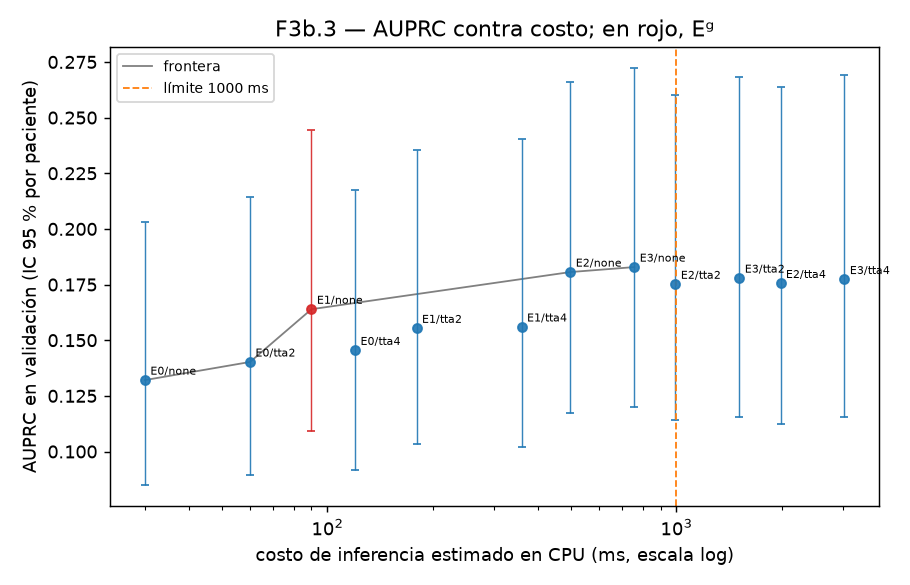
\includegraphics[width=\linewidth]{f3b_auprc_vs_cost}\\
      {\footnotesize En rojo, el ensamble elegido. Todo sobre validación.}
    \end{column}
  \end{columns}
\end{frame}

\begin{frame}{Calibración y umbral de decisión}
  \begin{columns}[T]
    \begin{column}{0.48\textwidth}
      \begin{block}{Calibración de Platt}
        El peso a la clase positiva \textbf{infla} las probabilidades. Una regresión logística sobre el logit, ajustada en validación, las devuelve a la escala real.
      \end{block}
      \begin{center}
        \small
        \begin{tabular}{lcc}
          \toprule
          \textbf{Ensamble, validación} & \textbf{Antes} & \textbf{Después} \\
          \midrule
          Brier & 0.0898 & \textbf{0.0161} \\
          ECE (error de calibración) & 0.1288 & \textbf{0.0022} \\
          \bottomrule
        \end{tabular}
      \end{center}
      \small El orden de las imágenes no cambia: el AUC es el mismo.
    \end{column}
    \begin{column}{0.48\textwidth}
      \begin{block}{Umbral $\tau_{95}$: sensibilidad $\geq 0.95$}
        Un melanoma no detectado cuesta más que una consulta de más.
        \begin{itemize}
          \item Fijado sobre \textbf{validación}, antes de abrir la prueba.
          \item Mediana de 2,000 remuestreos por paciente: con 88 melanomas, un solo corte dependería de cuatro casos.
          \item $\tau_{95} = 0.0039$: se refiere toda lesión con probabilidad mayor que \textbf{0.39\,\%}.
        \end{itemize}
      \end{block}
    \end{column}
  \end{columns}
  \vspace{0.4em}
  \begin{center}
    \small El umbral parece bajo porque la tasa base es 1.6\,\%: una lesión con 8\,\% ya tiene cinco veces el riesgo promedio.
  \end{center}
\end{frame}

% ============================================================
% RESULTADOS
% ============================================================
\begin{frame}{Resultados en el conjunto de prueba}
  \begin{columns}[c]
    \begin{column}{0.62\textwidth}
      \footnotesize\setlength{\tabcolsep}{4pt}
      \begin{tabular}{lcc}
        \toprule
        & \textbf{Modelo único} & \textbf{Ensamble} \\
        \midrule
        AUC-ROC & 0.834 [0.795, 0.872] & \textbf{0.843} [0.804, 0.881] \\
        AUPRC & 0.096 [0.065, 0.154] & \textbf{0.113} [0.076, 0.179] \\
        Sensibilidad en $\tau_{95}$ & 0.965 & \textbf{0.977} \\
        Especificidad en $\tau_{95}$ & \textbf{0.428} & 0.393 \\
        Melanomas detectados & 83 de 86 & \textbf{84 de 86} \\
        \bottomrule
      \end{tabular}
      \vspace{0.6em}

      \footnotesize 5,252 imágenes, 86 melanomas, 540 pacientes. Intervalos del 95\,\% por remuestreo a nivel paciente.

      \vspace{0.6em}
      \small
      \begin{itemize}
        \item La mejora del ensamble es \textbf{modesta} y los intervalos se traslapan.
        \item Criterio fijado antes de abrir la prueba: desplegar el ensamble si no es peor en AUC-ROC ni en AUPRC. \textbf{Se cumplió.}
      \end{itemize}
    \end{column}
    \begin{column}{0.35\textwidth}
      \centering
      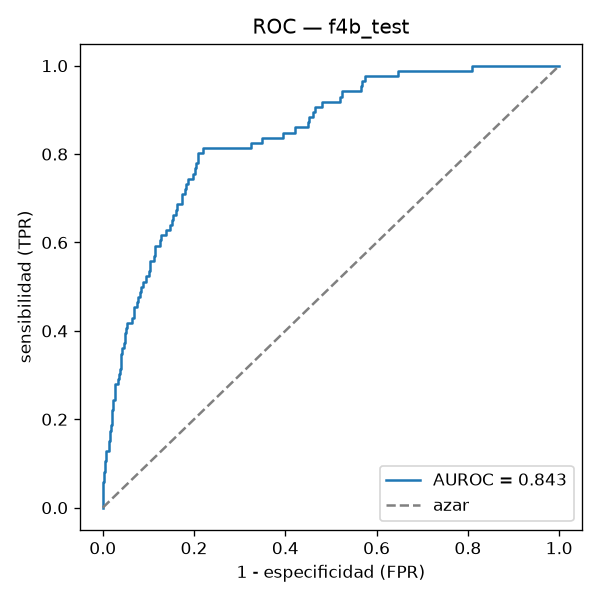
\includegraphics[width=\linewidth]{f4b_test_roc}
    \end{column}
  \end{columns}
\end{frame}

\begin{frame}{Punto de operación: qué significa en la práctica}
  \begin{columns}[c]
    \begin{column}{0.46\textwidth}
      \centering
      \small
      \textbf{Ensamble en $\tau_{95}$, conjunto de prueba}\\[0.5em]
      \begin{tabular}{lrr}
        \toprule
        & \textbf{No referir} & \textbf{Referir} \\
        \midrule
        Benigno real & 2,028 & 3,138 \\
        Melanoma real & \textbf{2} & \textbf{84} \\
        \bottomrule
      \end{tabular}
      \vspace{0.8em}

      \begin{tabular}{lr}
        \toprule
        Sensibilidad & \textbf{97.7\,\%} \\
        Especificidad & 39.3\,\% \\
        Valor predictivo positivo & 2.6\,\% \\
        Valor predictivo negativo & \textbf{99.9\,\%} \\
        \bottomrule
      \end{tabular}
    \end{column}
    \begin{column}{0.50\textwidth}
      \begin{block}{Lectura}
        \begin{itemize}
          \item Se detectan \textbf{84 de 86} melanomas.
          \item Se refiere el \textbf{61\,\%} de las lesiones; de ellas, 1 de cada 38 es melanoma.
          \item De las \textbf{no} referidas, 2 de 2,030 eran melanoma.
        \end{itemize}
      \end{block}
      \begin{alertblock}{El precio de la sensibilidad alta}
        Muchos falsos positivos. Por eso el sistema sirve para \textbf{priorizar}, no para descartar ni para diagnosticar.
      \end{alertblock}
    \end{column}
  \end{columns}
\end{frame}

\begin{frame}{¿Cómo leer un AUPRC de 0.113?}
  \begin{block}{Contra el azar}
    Con 1.64\,\% de melanomas en la prueba, un clasificador aleatorio obtiene AUPRC $\approx 0.016$. El ensamble alcanza \textbf{0.113: unas siete veces más}.
  \end{block}
  \vspace{0.5em}
  \textbf{Contra la literatura (AUC-ROC)}
  \begin{center}
    \small
    \begin{tabular}{lcl}
      \toprule
      \textbf{Referencia} & \textbf{AUC-ROC} & \textbf{Condiciones} \\
      \midrule
      Ha et al. (2020), ganador del reto & 0.949 & 18 modelos, hasta 896 px, datos de 2018 y 2019, metadatos \\
      Cassidy et al. (2022) & 0.80 & Modelo único, ISIC 2020 sin duplicados \\
      \textbf{Este trabajo} & \textbf{0.843} & 3 modelos a 224 px, solo ISIC 2020, GPU gratuita \\
      \bottomrule
    \end{tabular}
  \end{center}
  \vspace{0.3em}
  \begin{itemize}
    \item Los conjuntos de evaluación \textbf{no son los mismos}: la comparación ubica, no clasifica.
    \item Validación contra prueba (modelo único): AUC-ROC 0.834 en ambas; AUPRC 0.132 contra 0.096. Esa caída es la \textbf{brecha de generalización}, y por eso se reporta la prueba.
  \end{itemize}
\end{frame}

\begin{frame}{Evaluación externa: DDI (Diverse Dermatology Images)}
  \begin{columns}[T]
    \begin{column}{0.50\textwidth}
      \small
      \textbf{656 fotografías clínicas} con biopsia, etiquetadas por tono de piel (Fitzpatrick). Maligno contra benigno, modelo único.
      \vspace{0.5em}
      \begin{center}
        \setlength{\tabcolsep}{4pt}
        \begin{tabular}{lrc}
          \toprule
          \textbf{Grupo} & \textbf{n} & \textbf{AUC-ROC} \\
          \midrule
          Todas & 656 & 0.596 [0.541, 0.648] \\
          Fitzpatrick I--II & 208 & 0.590 \\
          Fitzpatrick III--IV & 241 & 0.596 \\
          Fitzpatrick V--VI & 207 & 0.604 \\
          \bottomrule
        \end{tabular}
      \end{center}
      \vspace{0.3em}
      Referencia: tres algoritmos publicados obtuvieron 0.56 a 0.67 sobre las mismas imágenes (Daneshjou et al., 2022).
    \end{column}
    \begin{column}{0.46\textwidth}
      \begin{alertblock}{Fuera de su dominio, el modelo no sirve}
        \begin{itemize}
          \item El AUC-ROC cae de 0.83 a \textbf{0.60}.
          \item La calibración se pierde (ECE 0.23).
          \item El umbral refiere casi todo (especificidad 0.01).
        \end{itemize}
      \end{alertblock}
      \begin{block}{Sobre el tono de piel}
        Desempeño similar entre grupos, pero \textbf{bajo en todos}. Cambian a la vez el tipo de imagen y la tarea: \textbf{no se puede concluir} sobre equidad.
      \end{block}
    \end{column}
  \end{columns}
\end{frame}

% ============================================================
% EXPLICABILIDAD
% ============================================================
\begin{frame}{Explicabilidad: mapas de activación (Grad-CAM)}
  \begin{columns}[c]
    \begin{column}{0.50\textwidth}
      \centering
      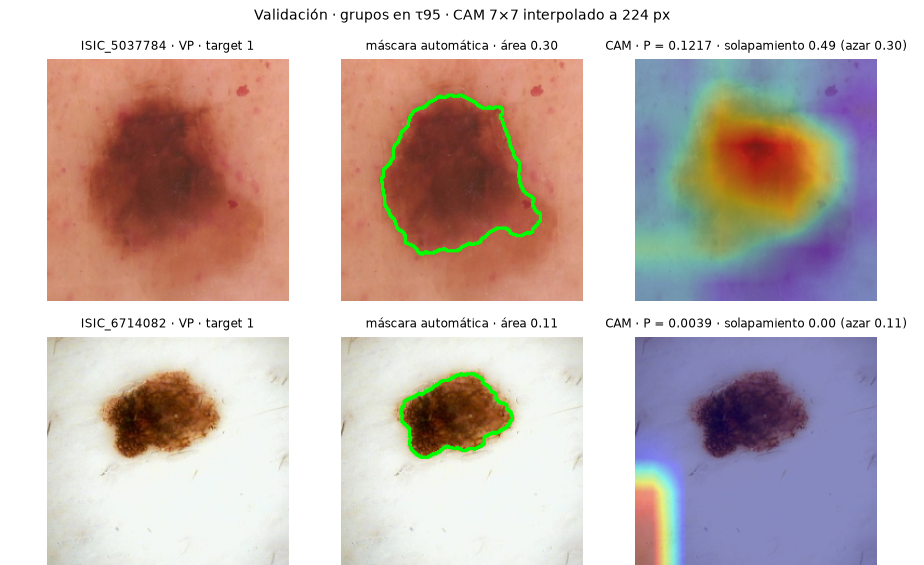
\includegraphics[width=\linewidth]{cam_tp}\\
      {\footnotesize Dos melanomas referidos: imagen, máscara automática y mapa.}
    \end{column}
    \begin{column}{0.47\textwidth}
      \small
      \textbf{¿Por qué?} Sin una explicación, una probabilidad sola no genera confianza ni permite detectar fallas.
      \vspace{0.4em}
      \begin{itemize}
        \item \textbf{Verificado}: equivale a CAM (correlación 1.000 en 50 imágenes) y \textbf{depende de los pesos} (prueba de cordura de Adebayo et al.).
        \item Malla de $7 \times 7$: señala \textbf{regiones}, no estructuras finas.
      \end{itemize}
      \vspace{0.2em}
      \begin{alertblock}{Hallazgo}
        En los melanomas detectados, solo el \textbf{22\,\%} de la activación cae dentro de la lesión, contra 19\,\% esperado por azar. El modelo también se apoya en la \textbf{piel que la rodea}.
      \end{alertblock}
    \end{column}
  \end{columns}
\end{frame}

\begin{frame}{Sensibilidad a artefactos}
  \begin{center}
    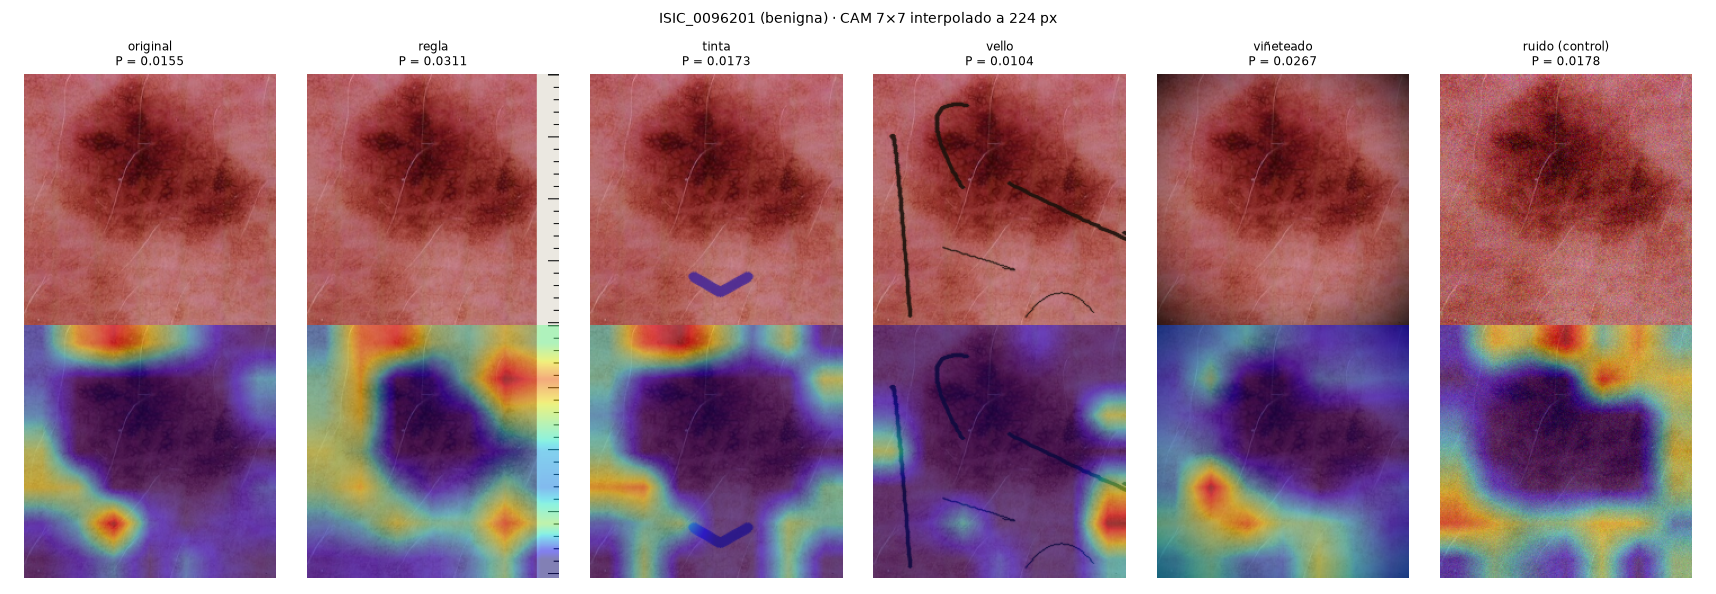
\includegraphics[width=0.78\linewidth]{f5_artifact_panel}
  \end{center}
  \vspace{-0.4em}
  \begin{columns}[T]
    \begin{column}{0.48\textwidth}
      \small
      \textbf{Experimento}: a 1,000 lesiones benignas y 88 melanomas de validación se les añade un artefacto sintético y se compara contra un control de ruido.
    \end{column}
    \begin{column}{0.48\textwidth}
      \small
      \begin{itemize}
        \item \textbf{Tinta}: el 84\,\% de las benignas no referidas pasa a referirse (71\,\% con el control).
        \item \textbf{Ruido o vello}: 14 a 16 de 84 melanomas dejan de referirse.
      \end{itemize}
    \end{column}
  \end{columns}
  \vspace{0.3em}
  \begin{center}
    \small Coincide con lo reportado por Winkler et al. (2019) en un sistema comercial: la calidad de la imagen importa.
  \end{center}
\end{frame}

% ============================================================
% SISTEMA
% ============================================================
\begin{frame}{Sistema: API e interfaz web}
  \begin{center}
    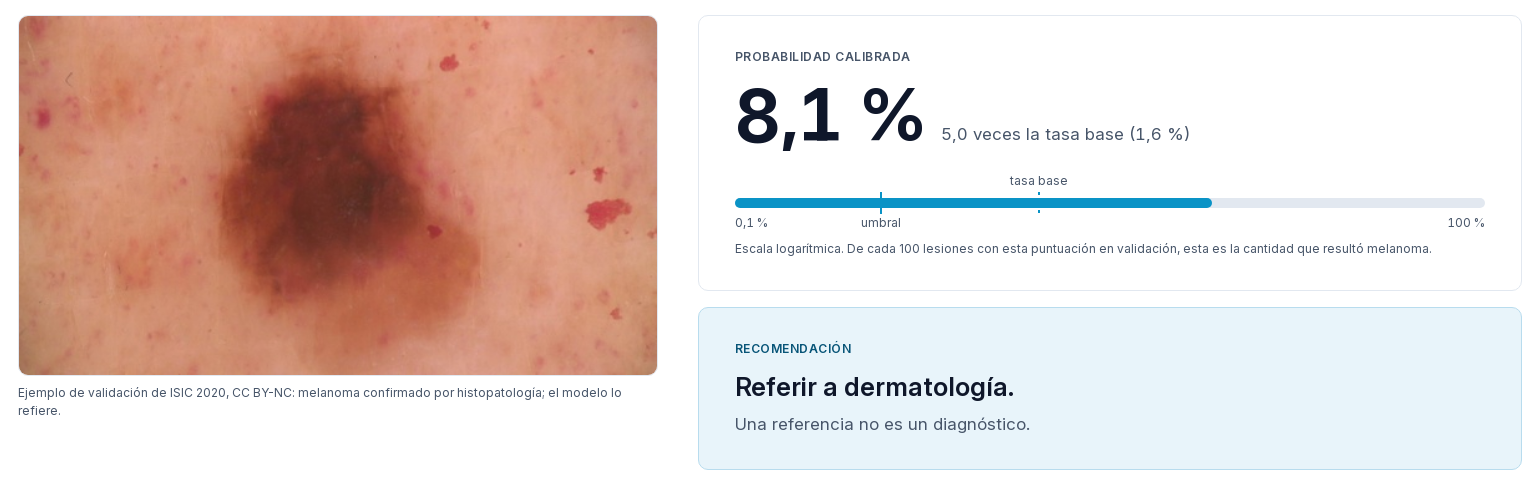
\includegraphics[width=0.66\linewidth]{ui_resultado}
  \end{center}
  \vspace{-0.6em}
  \footnotesize
  \begin{columns}[T]
    \begin{column}{0.32\textwidth}
      \textbf{Paquete de modelo}
      \begin{itemize}
        \item Tres redes en \textbf{ONNX}, calibración y umbrales, con SHA256.
        \item Paridad con PyTorch: diferencia máxima $2.2 \times 10^{-5}$.
      \end{itemize}
    \end{column}
    \begin{column}{0.30\textwidth}
      \textbf{API} (FastAPI, sin PyTorch)
      \begin{itemize}
        \item Imagen Docker de \textbf{437 MB}.
        \item Latencia en CPU: mediana \textbf{99 ms}, p95 118 ms.
      \end{itemize}
    \end{column}
    \begin{column}{0.32\textwidth}
      \textbf{Interfaz} (React)
      \begin{itemize}
        \item Probabilidad junto a la \textbf{tasa base}.
        \item Dice «referir» o «no referir»; \textbf{nunca «benigna»}.
      \end{itemize}
    \end{column}
  \end{columns}
\end{frame}

% ============================================================
% CONCLUSIONES
% ============================================================
\begin{frame}{Conclusiones}
  \begin{enumerate}
    \item \textbf{Objetivo alcanzado}: un clasificador de melanoma evaluado sobre un conjunto de prueba bloqueado, con probabilidades calibradas, explicabilidad validada y una interfaz funcional.
    \item \textbf{Desempeño}: AUC-ROC de \textbf{0.843} y AUPRC de \textbf{0.113} (siete veces el azar); en el punto de operación detecta \textbf{84 de 86} melanomas con una especificidad de 39\,\%.
    \item \textbf{El rigor cambia la cifra}: sin exactitud ni datos balanceados artificialmente, las métricas son menos vistosas, pero describen el problema real.
    \item \textbf{Los resultados negativos también son resultados}: la resolución, la aumentación en inferencia y los metadatos no aportaron; fuera de dermatoscopía el modelo no generaliza.
  \end{enumerate}
  \begin{exampleblock}{Veredicto}
    El sistema es una \textbf{herramienta educativa de apoyo a la priorización}. No es un dispositivo de diagnóstico y no debe usarse para tomar decisiones clínicas.
  \end{exampleblock}
\end{frame}

\begin{frame}{Limitaciones a considerar}
  \begin{enumerate}
    \item \textbf{Muchos falsos positivos}: valor predictivo positivo cercano al 3\,\%; sirve para priorizar, no para descartar.
    \item \textbf{Muestra pequeña}: 86 melanomas en la prueba; el intervalo del AUC-ROC mide $\pm 0.04$ y los subgrupos son solo exploratorios.
    \item \textbf{Generalización}: no funciona con fotografías clínicas (AUC-ROC 0.60 en DDI).
    \item \textbf{Solo melanoma}: una probabilidad baja no descarta otros cánceres de piel.
    \item \textbf{Población}: datos retrospectivos de Europa, Estados Unidos y Australia; sin pacientes mexicanos.
    \item \textbf{Artefactos y calidad de imagen}: la tinta y el ruido cambian la decisión.
    \item \textbf{Sin aprobación regulatoria} ni evaluación prospectiva.
  \end{enumerate}
  \vspace{0.4em}
  \begin{center}
    \small\textit{Declarar el alcance real del modelo es parte de construirlo con responsabilidad.}
  \end{center}
\end{frame}

\begin{frame}{Trabajo futuro}
  \begin{itemize}
    \item \textbf{Más datos}: incorporar otros años de ISIC para aumentar los casos positivos, cuidando la separación por paciente.
    \item \textbf{Robustez a artefactos}: recortar o segmentar la lesión antes de clasificar; en Winkler et al. el recorte revirtió el efecto de la tinta.
    \item \textbf{Validación local}: evaluación prospectiva con población mexicana y con los equipos de una clínica real.
    \item \textbf{Despliegue}: publicar la demostración en internet (en curso).
    \item \textbf{Nuevo conjunto de prueba}: el presupuesto de accesos está agotado; cualquier mejora futura necesita datos nuevos para evaluarse sin sesgo.
  \end{itemize}
\end{frame}

\begin{frame}[plain]
  \begin{center}
    {\huge\bfseries\color{azulfi} Gracias}\\[1.2em]
    {\large ¿Preguntas?}\\[2em]
    \textbf{Edgar Eduardo Ontiveros Lara}\\
    \texttt{\correo}\\[1em]
    \small Universidad Autónoma de Chihuahua --- Facultad de Ingeniería\\[2.6em]
    
\includegraphics[height=12mm]{logo_uach}\hspace{6.8cm}
\includegraphics[height=12mm]{logo_fi}
  \end{center}
\end{frame}

\end{document}
